\documentclass{beamer}

\usepackage{caption,subcaption}
\usepackage{pgf,tikz}
\usepackage{pgfplots}
\usepackage{tikz-3dplot}
\usetikzlibrary{shapes.geometric,arrows.meta,decorations.pathreplacing}

\title{Differential Geometry}
\author{Module I}
\institute{Chapter 5 : Vector Fields on Surfaces, Orientation}

\begin{document}

\begin{frame}
\maketitle
\end{frame}

\begin{frame}{Vector Fields on Surfaces}
\begin{definition}[Vector Field on a surface]
\begin{itemize}
	\item $n$-Surface, $S \subset \mathbb{R}^{n+1}$ 
	\item Vector Field on $S$, $\mathbf{X}(p) = (p,X(p)),\ \forall p \in S$\\
		where $X : S \to \mathbb{R}^{n+1} \implies X(p) \in \mathbb{R}^{n+1} \implies \mathbf{X}(p) \in \mathbb{R}_p^{n+1}$
\end{itemize}
\end{definition}

\begin{exampleblock}{Vector Field on $1$-sphere}
	$f(x,y) = x^2+y^2$ and $S = f^{-1}(1) \subset \mathbb{R}^2$\\
	$\nabla f(a,b) = (a,b,2a,2b) \ne (x,y,0,0),\ \forall (x,y) \in S$\\
\end{exampleblock}

\begin{figure}
\captionsetup[subfigure]{position=above}
\begin{subfigure}{0.3\textwidth}
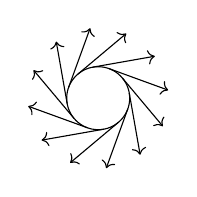
\begin{tikzpicture}[scale=0.4]
	\draw (0,0) circle (1cm);
	\foreach \x in {10,40,...,360}
		{\draw[->] ({cos(\x)},{sin(\x)}) -- ({cos(\x)+2*sin(\x)},{sin(\x)-2*cos(\x)}); }
\end{tikzpicture}
\subcaption{$X(x,y) = (2y,-2x)$}
\end{subfigure}
\begin{subfigure}{0.3\textwidth}
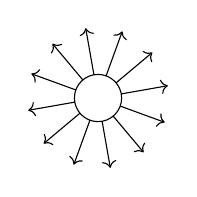
\begin{tikzpicture}[scale=0.3]
	\draw (0,0) circle (1cm);
	\foreach \x in {10,40,...,360}
		{\draw[->] ({cos(\x)},{sin(\x)}) -- ({3*cos(\x)},{3*sin(\x)}); }
\end{tikzpicture}
\subcaption{$X(x,y) = (2x,2y)$}
\end{subfigure}
\begin{subfigure}{0.3\textwidth}
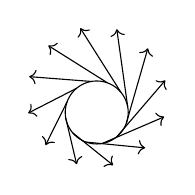
\begin{tikzpicture}[scale=0.4]
	\draw (0,0) circle (1cm);
	\foreach \x in {10,40,...,360}
		{\draw[->] ({cos(\x)},{sin(\x)}) -- ({cos(\x)-2*sin(\x)},{sin(\x)+2*cos(\x)+0.5}); }
\end{tikzpicture}
\subcaption{$X(x,y) = (-2y,2x+0.5)$}
\end{subfigure}
\caption{Vector Fields over $1$-sphere}
\end{figure}
\end{frame}

\begin{frame}{Smooth Vector Field over a Surface}
\begin{block}{Vector Field and Surface}
\begin{itemize}
	\item $n$-surface, $S= f^{-1}(c) \subset \mathbb{R}^{n+1}$\\
		where $f : U \to \mathbb{R}$ and $\nabla f(p) \ne 0,\ \forall p \in S$
	\item Vector Field, $\mathbf{X}(p) = (p,X(p))$, where $\mathbf{X}(p) \in \mathbb{R}_p^{n+1}$ and
	\item Associated function, $X : S \to R^{n+1}$
\end{itemize}
\end{block}
\begin{definition}[Smooth Vector Field over Surface]
	$\mathbf{X}$ on $S$ is \textbf{smooth} if the associated function $X$ has a smooth extension to an open set containing $S$
\begin{itemize}
	\item $\exists \text{ open set }V,\ S \subset V \subset U \subset \mathbb{R}^{n+1}$ and 
	\item $\exists \tilde{X} : V \to R^{n+1}$ is smooth\\
		where $\tilde{X} : V \to R^{n+1},\  X(p) = \tilde{X}(p),\ \forall p \in S$
\end{itemize}
\end{definition}
\end{frame}

\begin{frame}{Unique Integral Curve on Surface}
\begin{theorem}[Maximal, Integral Curve on Surface]
\begin{itemize}
	\item $\mathbf{X}$ smooth, tangent vector field on $n$-surface $S$
	\item $\forall p \in S$
	\item $\exists$ open interval $I$ containing $0$ and
	\item $\exists$ parameterised curve $\alpha : I \to S$ such that there exists\\
		a unique, maximal, integral curve on $S$ through $p$
	\begin{itemize}
		\item $\alpha(0) = p$
		\item $\dot{\alpha}(t) = \mathbf{X}(\alpha(t)),\ \forall t \in I$
		\item $\beta : \tilde{I} \to S$ such that $\tilde{I} \subset I$ and $\beta(t) = \alpha(t),\ \forall t \in \tilde{I}$
	\end{itemize}
\end{itemize}
\end{theorem}
\end{frame}

\begin{frame}{Proof : Maximal, Integral Curve on Surface}
\begin{itemize}
	\item Smooth, Vector Field $\mathbf{X}$ on $S$
	\begin{itemize}
		\item $\mathbf{X}$ on $S$ is smooth, then extension $\tilde{X}$ smooth on open set $V$
		\item $S$ is $n$-surface, then we have open set $U$ such that\\
			$f : U \to \mathbb{R}$, $S = f^{-1}(c) \subset U$, and $\nabla f(p) \ne 0,\ \forall p \in S$
	\end{itemize}
	\item Smooth, Vector Field on an open set $W$ containing $S$\\
		$ W = \{ q \in U \cap V : \nabla f(q) \ne 0 \} $
		$$ \mathbf{Y}(q) = \tilde{\mathbf{X}}(q) -\frac{\tilde{\mathbf{X}}(q) \cdot \nabla f(q)}{\|\nabla f(q)\|^2}\nabla f(q),\ \forall q \in W $$
	\item Maximal Integral Curve $\alpha$ on $\mathbf{Y}$ through $p$ (Ref : Chap. 2)\\
		$\alpha : I \to W,\ \dot{\alpha}(t) = \mathbf{Y}(\alpha(t)),\forall t \in I$ and ${\color{red}\alpha(0) = p}$
	\item Maximal Integral Curve $\alpha$ on $S$ through $p$\\
		$ (f \circ \alpha)'(t) = \nabla f(\alpha(t)) \cdot \dot{\alpha}(t) = \nabla f(\alpha(t)) \cdot \mathbf{Y}(\alpha(t)) = 0 $ \\
		$p \in f^{-1}(c) \implies f(\alpha(0)) = c \implies f \circ \alpha(t) = c$\\
		$\implies \alpha(I) \subset f^{-1}(c) = S \implies {\color{red}\alpha : I \to S}$\\
		$\dot{\alpha}(t) = \mathbf{Y}(\alpha(t)) = \mathbf{X}(\alpha(t)) \implies {\color{red} \dot{\alpha}(t) = \mathbf{X}(\alpha(t))}$
\end{itemize}
\end{frame}

\begin{frame}{Connectedness and Components}
\begin{definition}[Connectedness]
	Subset $S$ of $\mathbb{R}^{n+1}$ is connected if for any $p,q \in S$, there a continuous function $\alpha : [a,b] \to S$ such that $\alpha(a) = p$ and $\alpha(b) = q$. {\color{purple}That is, there a path connecting any two points.}
\end{definition}

\begin{definition}[Connected Component]
	The equivalence classes of $S$ under connectedness are the connected components of an $n$-surface, $S$.
\end{definition}
\end{frame}
\begin{frame}{Orientation}
\begin{theorem}[Oriented $n$-surface]
\begin{itemize}
	\item $\forall$ connected $n$-surface, $S$
	\item $\exists$ two unit normal vector fields $\mathbf{N_1}, \mathbf{N_2}$ and
	\item $\mathbf{N_2}(p) = -\mathbf{N_1}(p),\ \forall p \in S$
\end{itemize}
\end{theorem}
\begin{proof}
\begin{itemize}
	\item $n$-surface $S$\\
		$\implies S = f^{-1}(c),\ f : U \to \mathbb{R},\ \nabla f(p) \ne 0,\ \forall p \in S$
		$$\mathbf{N_1}(p) = \frac{\nabla f(p)}{\|\nabla f(p) \|},\ \forall p \in S$$
	\item $\mathbf{N_2}(p) = -\mathbf{N_1}(p)$
	\item $\exists \mathbf{N_3} \in S_p^{\perp} \implies \mathbf{N_3}(p) = g(p)\mathbf{N_1}(p) = \pm \mathbf{N_1}(p)$
\end{itemize}
\end{proof}
\end{frame}

\begin{frame}{Orientation}
\begin{definition}[Orientation]
	A smooth, unit normal vector field on an $n$-surface $S$ is an \textbf{orientation} of $S$
\end{definition}
\begin{definition}[Oriented Surface]
\begin{itemize}
	\item $n$-surface, $S$
	\item an orientation of $S$, $\mathbf{N}$
\end{itemize}
\end{definition}
\begin{block}{M\"obius Band is not an $n$-surface}
\begin{itemize}
	\item M\"obius Band, $B$ doesn't have two orientations
	\item There doesn't exists a smooth function $f$ such that\\
		$B = f^{-1}(c),\ f : U \to \mathbb{R},\ \nabla f(p) \ne 0,\ \forall p \in B$
\end{itemize}
\end{block}
\end{frame}

\begin{frame}{Positive Tangent Direction}
\begin{definition}[direction]
	A unit vector in $\mathbb{R}_p^{n+1}$ is a \textbf{direction} at $p$
\end{definition}
\begin{definition}[Positive Tangent Direction]
\begin{itemize}
	\item $1$-surface/Plane Curve, $C$
	\item Orientation, $N$
	\item \textbf{Positive Tangent Direction} at $p$ is obtained by\\
		rotating orientation at $p$ by $-\pi/2$ in anticlockwise direction.
	\item If $N(p) = (x,y)$, then the positive tangent direction at $p$ is $T(p) = (-y,x)$ 
\end{itemize}
\end{definition}
\end{frame}

\begin{frame}{Positive $\theta$-Rotation}
\begin{definition}[Positive $\theta$-Rotation]
\begin{itemize}
	\item $2$-surface, $S$
	\item Orientation, $\mathbf{N}$
	\item Positive $\theta$-rotation, $R_\theta : S_p \to S_p$\\
		$R_\theta(\mathbf{v}) = \cos \theta \mathbf{v} + \sin \theta \mathbf{N}(p) \times \mathbf{v}$
	\item $R_\theta$ is the Right-handed rotation about $\mathbf{N}(p)$ through Angle $\theta$
\end{itemize}
\end{definition}
\end{frame}

\begin{frame}{Consistent Basis}
\begin{definition}[Consistent Basis]
\begin{itemize}
	\item $3$-surface $S$
	\item Orientation $\mathbf{N}$
	\item $\mathcal{B} = \{ \mathbf{e_1},\mathbf{e_2},\mathbf{e_3} \}$ be ordered basis for $S_p$
	\item Consistent Basis, $\mathcal{B}$ if
		$$\det \begin{pmatrix} \mathbf{e_1} \\ \mathbf{e_2} \\ \mathbf{e_3} \\ \mathbf{N}(p) \end{pmatrix} \text{ is positive} $$
		\item Inconsistent basis if determinant is negative.
\end{itemize}
\end{definition}
\end{frame}

\begin{frame}
	\vspace{0.6in}
	\hspace{3cm} {\color{blue}\Huge{Thank You}}
\end{frame}

\end{document}
